\documentclass[twocolumn,a4paper,10pt,preprint,3p]{elsarticle}

\usepackage{amsmath}
\usepackage{lineno,hyperref}
\usepackage{tabularx}
\usepackage{amssymb}
\usepackage{booktabs}
\usepackage{multirow}
\usepackage{caption,subcaption}
\usepackage[ruled,vlined]{algorithm2e}
\modulolinenumbers[5]

\journal{Journal of Web Semantics}

%% `Elsevier LaTeX' style
\bibliographystyle{elsarticle-num}

%%%%%%%%%%%%%%%%%%%%%%%

\begin{document}

% =========================================
% front matter

\begin{frontmatter}

\title{Adversarial Training for Knowledge Graph Embedding with Ensemble Construction}

% ----------------------
% affiliations

\author[hrbaddress]{Xiang Zhang}
\ead{xiang.zhang@nlpr.ia.ac.cn} % `ead' stands for email address

\author[hrbaddress]{Qingsong Meng}
\ead{mqs0530@163.com}

\author[ucasaddress]{Shizhu He}
\ead{shizhu.he@nlpr.ia.ac.cn}

\author[ucasaddress]{Kang Liu}
\ead{kliu@nlpr.ia.ac.cn}

\author[ucasaddress]{Jun Zhao\corref{correspondingauthor}}
\ead{jzhao@nlpr.ia.ac.cn}

\cortext[correspondingauthor]{Corresponding author}
\address[hrbaddress]{Harbin University of Science and Technology, No.52 Xuefu Road, Nangang District, Harbin, 150080, China}
\address[ucasaddress]{University of Chinese Academy of Sciences, No.19(A) Yuquan Road, Shijingshan District, Beijing, 100049, China}

% -------------------------
% abstract + keywords

\begin{abstract}
Adversarially training.
\end{abstract}

\begin{keyword}
Knowledge Graph \sep{} Representation Learning \sep{} Adversarial Training \sep{} Ensemble Learning
\MSC[2010] 68T30 \sep{} 68T50
\end{keyword}

\end{frontmatter}

% ==========================================
% main text

\linenumbers{}

% ------------------------
% introduction

\section{Introduction}
\label{sec:intro}

People devote to construct and organize broad-coverage knowledge graphs (KGs) such as WikiData, Freebase and WordNet. KGs contain inter-linked triplets, and a triplet ((head entity, relation, tail entity), simply as (h, r, t)) indicates the fact that the two entities hold the relation. The rich structured knowledge bases become useful resources to support downstream natural language processing (NLP) and artificial intelligence (AI) applications such as recommended system (加参考文献), Web Search (加参考文献) and Question Answering (加参考文献). Due to the knowledge represented with symbols, KGs cannot be easily embodied in downstream models, especially in neural network models. In addition, the knowledge reasoning (another core task in AI) with the symbolic representation are inflexible and inefficient.

\begin{figure}[htb]
    \centering
    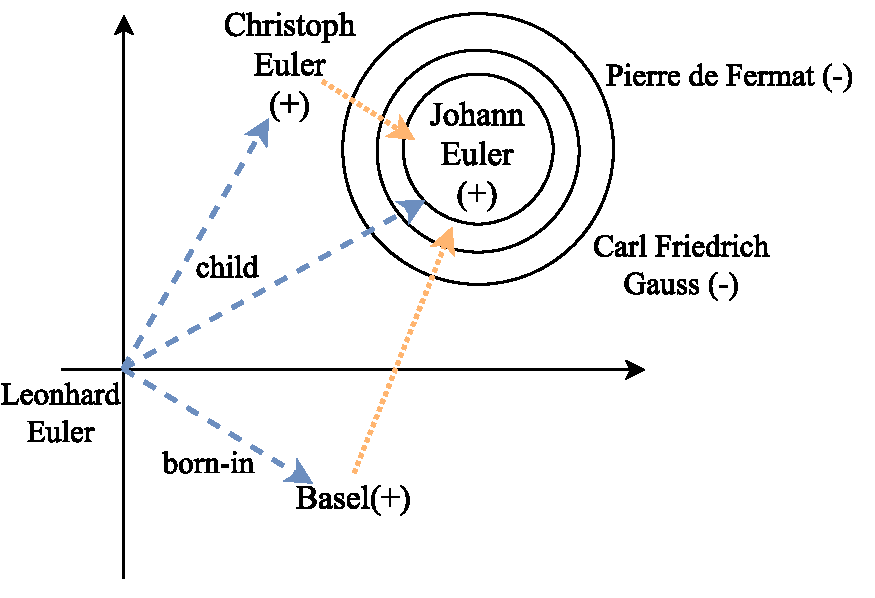
\includegraphics[width=0.3\textwidth]{images/translation.pdf}
    \caption{Translation example where \emph{Leonhard Euler} acts as the head entity. Blue arrows indicate the translation from the head to tail entities under the relation \emph{child} and \emph{born-in}. Orange arrows illustrate the improperness of randomly negative sampling. Replacing \emph{Johann Euler} with \emph{Basel} is too easy for the model to improve, while substitution with \emph{Christoph Euler} will mislead the training. The best strategy is to choose the close and false tail entities as negative samples, that is, \emph{Pierre de Fermat} and \emph{Carl Friedrich Gauss} denoted by a minus sign (-) in this figure.}
\label{translation-example}
\end{figure}

To better and conveniently utilize the knowledge, alike to the word embedding, knowledge graph embeddings (KGE) have been proposed to learn the representations of the elements and structures in a KG, which attempt to embed it into a low-dimensional continuous space.  Specifically, KGE aims to learn a numerical  representation for each \emph{entity} and \emph{relation} in the KG. Consider the following example. The triple \emph{(Leonhard Euler, born-in, Basel)} is a selected fact from a typical knowledge graph, \emph{WikiData}\footnote{https://www.wikidata.org/}. Typical KGE models assign a vectorized representation for the head entity \emph{Leonhard Euler} and the tail entity \emph{Basel}, and some models also give a representation for each relation, namely \emph{born-in} in this example. In general, there must be some characteristics to hold or constraints to meet for these representations, which facilitate other tasks like inference or completion on the knowledge graph.

One of the most popular constraints is the translation assumption. Borders et al.~\cite{TransE2013} first proposed the \emph{TransE} model, in which the representation of a tail entity~$(t)$ could be arithmetically computed from the head entity~$(h)$ and relation~$(r)$, that is, $h + r \simeq t$. This gives a very concise and beautiful geometric explanation that every relation can move or \emph{translate} an entity embedding into another, translating \emph{Leonhard Euler} into \emph{Basel} in Figure~\ref{translation-example} for example, and hence its name \emph{TransE}.
The model is trained by minimize a hinge loss with a predefined margin between the distances of positive and negative samples. The distance in TransE is given by an L1 or L2 norm of the vector~$h + r - t$, which is a special case of scoring (or~energy) function.

Models that share the same framework but differ in the scoring function can be seen as the \textbf{discriminative approach}. For instance, \emph{TransR}~\cite{TransR2015} introduces a mapping from the entity space to the relation space under the translation assumption, where the scoring functions is $\lVert h M_r + r - t M_r \rVert_2^2 $, and \emph{Neural Tensor Network} (NTN)~\cite{NTN} utilizes a bilinear model and a single layer neural network to construct the scoring function. The crucial scoring function within these models aims to predict high scores for real facts in a knowledge graph while lower the scores of the sampled negative facts, thus we may expect it to give a reasonably high score for some missing but possible facts at testing time.

Despite the success of these discriminative models, there are two challenges remaining for the problem.
The first one is the \textbf{improperness of negative sampling}, that the randomly chosen negative samples can be either completely absurd or indeed authentic.
The model can differentiate with little effort the absurd samples which are therefore useless for training. But the authentic negative samples will fool the model and mislead it towards a wrong direction. Figure~\ref{translation-example} gives an illustration. For these two facts in WikiData \emph{(Leonhard Euler, child, Chistoph Euler)} and \emph{(Leonhard Euler, child, Johann Euler)}, we may simply substituting the tail entity by another absurd entity, say, \emph{Basel} to construct a negative sample, which yields a triple \emph{(Leonhard Euler, child, Basel)}. The model will receive no improvement because the entity is even a city rather than a person. But if an either child is selected to act as the tail entity for the other triple which further serves as a negative sample, the model will probably get fooled.

\begin{table}
    \centering
    \begin{tabular}{c|r|r}
        \toprule
        Percentile & FB15k & WN18 \\
        \midrule
        25\% &  1   & 1  \\
        50\% &  1   & 1 \\
        75\% &  2   & 1 \\
        90\% &  5   & 2 \\
        99\% &  28  & 10 \\
        max & 3590  &  471 \\
        \midrule
        mean &  3.14 & 1.65 \\
        count & 153630 & 85532 \\
        standard deviation & 18.36 & 5.08 \\
        \bottomrule
    \end{tabular}
    \caption{Statistics of tail entities given the same head entity and relation pair in the training data. Both the FB15k and WN18 dataset have a much greater mean than 1. At least 25\% distinct pairs of head entity and relation in FB15k (and at least 10\% in WN18) have more than 1 tail entity, which shows the ubiquitous presence of one-to-many relations. }
\label{one-to-many}
\end{table}

The second challenge is the \textbf{ubiquitous presence of the one-to-many relations}. These relations share the same head entity but move it to different tails, as the two children of Euler in the example of Figure~\ref{translation-example}.
Statistics in Table~\ref{one-to-many} shows that a large portion of relations from training data shows the one-to-many characteristic.
As we know, discriminative models give a score to every single new triple, but lack the ability to predict the entity probabilistic distribution in a global view.
Since the data is always incomplete and the real distribution is unknown, scoring function on its own may become entangled in pervasive one-to-many relations.
To better determine whether a missing and in particular one-to-many relation is possible or not, many previous work designed delicate models that is either very expressive neural network~\cite{NTN} or introduces mappings between entity and relation spaces~\cite{TransH2014,TransR2015,TransD}.
It's no doubt difficult to design an even better  discriminative model. From the other perspective, Xiao et al.~\cite{TransG} novelly proposed \emph{TransG} as a \textbf{generative model} to deal with the multi-semantic phenomenon in many one-to-many relations. While it still requires the traslation assumption to hold, TransG sheds lights on using the generative approach for this task, along with its theoritical framework and ability to incorporate complex prior and to explain the intrinsic patterns within data.

Inspired by the success of GAN~\cite{GAN}, we propose an adversarial ranking method to unify the generative and discriminative approaches, which simultaneously learns a discriminator and a generator to tackle the challenges above. The generator could predict the conditional probability distribution, while the discriminator would still function as previous models.

At the generator side, we discard the translation assumption. For simplicity, we just assume the head and relation are both uniformly distributed, thus concentrate on directly modeling the conditional probability $p(t\mid h, r)$ which generates the tail entity given its head and relation. As the generator is getting better, it would predict better entities as negative samples which is more useful for the discriminator than those randomly chosen ones, thus cures the problem of absurd negative sample.

At the discriminator side, inspired by the idea from IRGAN~\cite{IRGAN}, we build a ranking-based loss which will not take generated samples as complete negative samples but only give them lower rank compared to the positive sample.

We have talked about the traits of the discriminative and generative models in this task. Note that the generator can do much more than generating negative samples, it also has the power of prediction just like the discriminator. Empirically we know neither model could completely beat the opposite. The characteristics of these two are quite different and we thus have two very heterogeneous models in the adversarial training setting, which happens to meet the requirement for ensemble learning. Therefore we adopt a simple weighted voting method to ensemble the two only models and received very impressive results.

Our contributions are thus two-fold:
\begin{itemize}
    \item We propose an adversarial ranking training for representation learning of knowledge graph, in order to generate better negative samples and make better use of them.
    \item To exploit the power of both the generator and discriminator, we propose to use a simple ensemble method which beats all the baselines and achieves the best result.
\end{itemize}



% ---------------------------------------
% method

\begin{algorithm*}[t]
\DontPrintSemicolon
\KwData{$G=(X,U)$ such that $G^{tc}$ is an order.}
\KwResult{$G’=(X,V)$ with $V\subseteq U$ such that $G’^{tc}$ is an interval order.}
\Begin{
    $V \longleftarrow U$\;
    $S \longleftarrow \emptyset$\;
    \For{$x\in X$}{
    $NbSuccInS(x) \longleftarrow 0$\;
    $NbPredInMin(x) \longleftarrow 0$\;
    $NbPredNotInMin(x) \longleftarrow |ImPred(x)|$\;
    }
    \If{$NbPredInMin(x) = 0$ {\bf and} $NbPredNotInMin(x) = 0$}{
        $AppendToMin(x)$
    }
    
    \While{$S \neq \emptyset$}{
        remove $x$ from the list of $T$ of maximal index\;
        \While{$|S \cap  ImSucc(x)| \neq |S|$}{
            \For{$ y \in  S-ImSucc(x)$}{
                \{ remove from $V$ all the arcs $zy$: \} \;
                \For{$z \in  ImPred(y) \cap  Min$}{
                    remove the arc $zy$ from $V$\;
                    $NbSuccInS(z) \longleftarrow NbSuccInS(z) - 1$\;
                    move $z$ in $T$ to the list preceding its present list\;
                    \{i.e. If $z \in T[k]$, move $z$ from $T[k]$ to
                    $T[k-1]$\}
                }
                $NbPredInMin(y) \longleftarrow 0$\;
                $NbPredNotInMin(y) \longleftarrow 0$\;
                $S \longleftarrow S - \{y\}$\;
                $AppendToMin(y)$\;
            }
        }
        $RemoveFromMin(x)$\;
    }
}
    \caption{IntervalRestriction\label{IR}}
\end{algorithm*}

\section{Methods}

We formulate our adversarial training setting in this section. As stated in the previous section, our model consists of a discriminator and a generator, which are adversarially trained and exploited together through an ensemble method. We report each components in the following subsections.

\subsection{Notations}

A knowledge graph $\mathcal{K}$ can be defined as a triple $(\mathcal{E}, \mathcal{R}, \mathcal{F})$, where $\mathcal{E}$ is the set of entities, $\mathcal{R}$ is the set of relations, and $\mathcal{F}$ is the set of facts. Every fact $f\in \mathcal{F}$ is again a triple $(h, r, t), \forall h,t\in\mathcal{E}, r\in\mathcal{R}$. The training data $X$ is a subset of the real facts, $X \subset \mathcal{F}$.

We defined the discriminator $d$ as a scoring function which maps a triple to a scalar, namely $d: \mathcal{F}\rightarrow \mathbb{R}$. The generator on the contrary tries to maximize the joint probability $p(h, r, t)$ which is proportional to the conditional distribution $p_g(t \mid h, r)$. We thus defined the generator as a function $g: \mathcal{E} \times \mathcal{R} \rightarrow \mathbb{R}^{\lvert \mathcal{E} \rvert}$.

\begin{figure}[t]
    \centering
    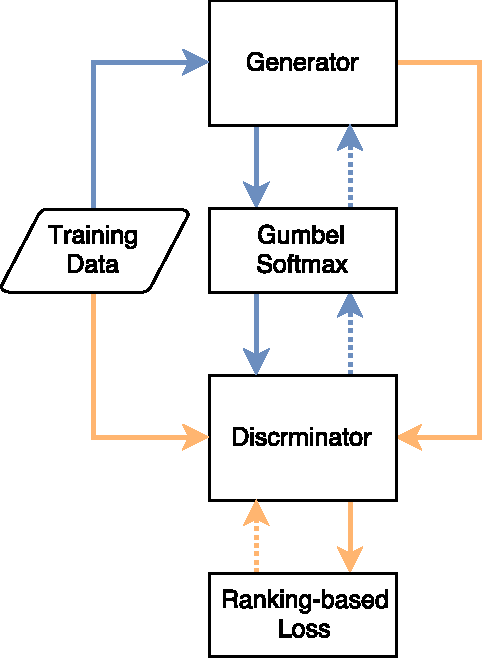
\includegraphics[width=0.35\textwidth]{images/overview.pdf}
    \caption{Overview of our adversarial training setting. The solid lines indicate the flow of training data and dash lines show the back propagation direction of gradients. Orange lines illustrate the process in which the discriminator uses generated negative samples and maximize the ranking-based objective. Blue lines shows the generator use discriminator as its feedback and propagate the gradient through gumbel softmax~\cite{GumbelSoftmax_Jiang_2016}.}
\label{system-overview}
\end{figure}

\subsection{Discriminator}

As discussed in the Section~\ref{sec:intro}, we use a ranking-based objective when training the discriminator. Here we defined the \emph{score distance} as follows,
\[
    sd(t, t^*; h, r) := \lvert d(h, r, t) - d(h, r, t^*) \rvert,
\]
where $h$ and $r$ are the head entity and relation respectively, $t$ is the tail entity from training data, and $t^*$ is a tail entity coming from either the generator or the training data, which making the score distance be 0 in the latter case.

We defined the ranking function as follows,
\begin{align*}
    rank_\tau(t, {\{\tilde t \}}_{i=1}^K)
    &= \frac{\exp(sd(t, t; h, r) / \tau)}
        {\sum_{t^*\in \{t\} \cup {\{\tilde t \}}_{i=1}^K } \exp (sd(t, t^*; h, r) / \tau) } \\
    &= \frac{1}
        {\sum_{t^*\in \{t\} \cup {\{\tilde t \}}_{i=1}^K } \exp (sd(t, t^*; h, r) / \tau) },
\end{align*}
where $t$ is a tail entity from the training data, $\tilde t$ is a tail entity sampled from the generator, $K$ indicates the number of tail entity samples in the ranking list, and $\tau$ is the temperature hyperparameter to control the variance of the softmax function.

We then define the training loss for the discriminator as follows,
\begin{align}
    \max_d \sum_{(h, r, t)\in X}
        &\mathbb{E}_{\tilde t_1, \dots, \tilde t_K \sim p_g(t \mid h, r)}
            rank_\tau(t, {\{\tilde t \}}_{i=1}^K) \notag \\
        &- \mathbb{E}_{\tilde t \sim p_g(t \mid h, r)}
            rank_\tau(\tilde t, t) \label{eq:d_loss}
\end{align}


Note the parameters of the discriminator only occur inside the expectation term. We can just draw samples from the distribution produced by the generator and feed them to the discriminator, and the optimization algorithm will work as it is intended to do. The orange lines in Figure~\ref{system-overview} illustrate the process.

\subsection{Generator}

The generator will output an probabilistic measure of the set of all entities $\mathcal{E}$. We minimize the following cross entropy term defined through the discriminators' feedback,

\begin{align}
    \min_g \sum_{(h, r, t)\in X}
        \mathbb{E}_{\tilde t \sim p_g(t \mid h, r)}
            \frac{\exp(d(h, r, \tilde t) / \tau)}
                 {\sum_{t^* \in \{ t, \tilde t\}} \exp(d(h, r, t^*) / \tau)} \label{eq:g_loss}
\end{align}

However, it's not possible to directly optimize the above loss function using gradient-based algorithms. In practice, we have to sample a discrete distribution, which makes a simple reparemeterization trick~\cite{VAE} fail. A popular solution to this problem is to adopt reinforcement learning. The REINFORCE algorithm~\cite{Williams_1992}, for example, reformulates the gradient of the generator objective above but is known to be hard to train and meets the problem of cold start. Furthermore, the gradients it produced tend to have high variance, though a baseline term was added in our experiments.

Since the generator actually gives a multinomial distribution, we adopt the gumbel softmax~\cite{GumbelSoftmax_Jiang_2016} which uses gumbel noise to reparemeterize the multinomial distribution. Specifically, we add standard gumbel noise to the unnormalized log probabilities (logits) and do softmax as follows,
\begin{align*}
    GumbelProb_i = \frac{\exp((logits_i + z_i)/ \tau)}{\sum_{j}\exp((logits_j + z_j)/ \tau)},
\end{align*}
where $z \sim Gumbel(0, 1)$ is the sampled gumbel noise, $logits$ is the output of the generator, and $\tau$ is the positive temperature. As $\tau$ descreases towards 0, the gumbel probability will approximate a one-hot vector sampled from the categorical distribution parameterized by the output logits, which is differentiable w.r.t.\ the $logits$. Blue lines in Figure~\ref{system-overview} illustrate the generator learning process, too.


\subsection{Pretraining and ensemble}

\paragraph{Pretraining} As GANs are hard to train, we introduce a pretraining procedure at first. Note the setting in previous subsections only works when the generator and discriminator are trained adversarially and alternatively. When it comes to the pretraining, we have to design new loss functions for them separately.

To keep things simple, we minimize the cross entropy loss for the generator as below,
\begin{equation}
    \min_g \sum_{(h, r, t)\in X} -p_g(t \mid h, r), \label{eq:g_pretrain}
\end{equation}.
Because our generator output logits only, we further use softmax to convert the logits to a normalized probability measure.

For the discriminator, we either use the similar hinge loss with margin as TransE~\cite{TransE2013},
\begin{equation}
    \min_d \sum_{\substack{(h, r, t)\in S,\\ (h^\prime, r, t^\prime)\in S^\prime }}
        {[ d(h, r, t) - d(h^\prime, r, t^\prime) + \gamma ]}_+, \label{eq:d_pretrain}
\end{equation}
where ${[\cdot]}_+$ denote the hinge loss, $\gamma$ is the margin hyperparameter. $S$ may either denotes the positive or negative samples. If we want the discriminator to give smaller scores for better samples, $S$ is the set of positive samples and $S'$ the set of negative ones, and vice vesa.

\paragraph{Ensemble} Construction of ensemble among base learners is beneficial to performance improvements~\cite{dietterich2000ensemble}. Because of the adversarial training setting, the discriminator and generator are two heterogeneous models and suitable for ensemble learning. We construct a simple weighted average method to exploits both models,
\begin{equation}
    s(h, r, t) = \alpha d(h, r, t) + (1 - \alpha) p_g(t \mid h, r), \label{eq:weighted-ensemble}
\end{equation}
where $\alpha$ is a hyperparameter tuned on the validation set.

% --------------------------------------
% related work

\section{Related work}

We continue to discuss the work related to ours and make comparisons with them in this section.

\paragraph{Translation models} As discussed in Section~\ref{sec:intro}, TransE~\cite{TransE2013} is a representative model adopting the translation assumption. Specifically, they try to minimize the following hinge loss,
\begin{equation}
    \min\sum_{\substack{(h, r, t)\in S,\\ (h^\prime, r, t^\prime)\in S^\prime }}
        {\left[\gamma + f(h, r, t) - f(h^\prime, r, t^\prime)\right]}_+, \label{eq:TransE}
\end{equation}
where $S$ is the set of triples and $S'$ is the set of negative samples. $f(h, r, t)$ can be viewed as an energy or scoring function which in their case is an L1 or L2 norm of $h + r - t$. TransH~\cite{TransH2014} extends the basic TransE by projecting entities to the hyperplaned defined by the relation. Let $\omega_r$ be the normal vector of the hyperplane, then the scoring function in TransH is defined as $f(h, r, t) = \lVert(h~-~\omega_r^T h \omega_r) + d_r -~(t~-~\omega_r^T t \omega_r)\rVert_2^2 $.
TransR~\cite{TransR2015} futher extends the idea by making the relation a complete space rather than a hyperplane in entity space. With a linear mapping between these two spaces, their scoring function is $f(h, r, t) = \lVert hM_r + r - h M_r \rVert_2^2$. These models differ from ours both in its discriminative nature and the translation assumption.

TransG~\cite{TransG} is a generative model and is thus closest to our work. It draws head and tail entities from gaussian distributions, and draw the relation from a mixture of both entities. It uses the Chinese restaurant process to model the relation token implying different semantics, namely the \emph{multi-semantic phenomenon}.
On the contrary, our model doesn't assume explicit gaussian density, but uses the adversarial framework to approximate the unknown real data distribution, which is a merit of GAN~\cite{Goodfellow_2016}.

\paragraph{Neural models} Apart from the translation-based scoring function, Structured Embedding~\cite{bordes2011structured_embedding} is the start of the other approach, which defines the scoring functions using two matrices as $f(h, r, t) = \lVert M_{r,1}h - M_{r,2}t \rVert_{L1}$. Latent Factor Model~\cite{jenatton2012bilinear} uses a bilinear model to characterize the relation between two entities with the scoring function as $f(h, r, t) = h^T W_r t$.
Single Layer Model is a baseline in Socher et al.~\cite{NTN}, which use one single layer neural network as the scoring function, namely $f(h, r, t)=u_r^T \tanh(W_r[h;t])$. They further propose the most expressive Neural Tensor Network (NTN) model, which utilizes the merits of both the bilinear model and single layer neural network. The scoring function is $u_r^T \tanh(h^T W_r^{[1:k]}t + V_r[h;t] + b_r)$. Due to the large amount of parameters, it's not easy to train NTN on large scale data.

\paragraph{GANs} Then let's move on to the GANs. GAN~\cite{GAN} proposes a vivid explaination of the minimax game between a discriminator and a generator, which is successfully applied to the image processing field~\cite{Ledig_2017_CVPR}. However, classic GAN is hard to train~\cite{Salimans_2016}. Through a detailed analysis on the objective, Arjovsky et al.\ proposed Wasserstein GAN~\cite{Arjovsky2017WGAN} which replaces the Jensen-Shannon divergence with the Earth-Mover distance. They also reported new techniques for training~\cite{Gulrajani2017LipschitzReg}, which aims to add penalty term into gradients to enforce the Lipschitz constraint.

In the field of natural language processing, SeqGAN~\cite{SeqGAN} is proposed to generate natural language sentences. They also use policy gradient method to backpropagate through discrete sampling. To evaluate the reward of generated sentences in advance, they use Monte Carlo tree search to roll out the whole sentence and use the reward to update in the middle of generation. RankGAN~\cite{RankGAN} futher extends the idea by incorporating the ranking-based loss, which tries to optimize the list-wise ranking of the generated sentence in a candidate list. The recently proposed IRGAN~\cite{IRGAN} nevertheless brings the adversarial training idea into the Information Retrieval field, which unifies both the discriminative and generative schools in a single framework. These models inspired us to use ranking as objective and to combine two models.

Tram\`er et al.~\cite{EnsembleAdvTraining} recently proposed a novel framework called Ensemble Adversarial Training. Along with the progress in using adversarial examples to attack trained models, they propose an extension of GAN that augments training data with perturbation using pretrained models, which is reminiscent of boosting methods in ensemble learning, while our method adopts the weighted average idea between the heterogeneously trained generator and discriminator.

Cai and Wang recently develops a similar KBGAN~\cite{Cai2017KBGAN} model to ours. They focus on using a generator to yield better negative samples for the training of discriminator, which uses a REINFORCE approach to propagate gradient back through stochastic sampling while we adopt the gumbel softmax reparameterization. Their method is flexible at using various models as the discriminator, theoritically even a non-differentiable one because of the power of reinforcement learning. On the contrary, we use GAN together with a ranking loss to deal with both kinds of improper negative samples mentioned in Section~\ref{sec:intro}. Furthermore, we also shows the usefulness of ensemble learning in this setting.


% --------------------------------------
% experiments

\begin{table}[hbtp]
    \centering
    \begin{tabular}{crr}
        \toprule
        Dataset & FB15k & WN18 \\
        \midrule
        entities &  14951   &  40943  \\
        relations &  1345   & 18 \\
        training set &  483142   & 141442 \\
        validation set &  50000   & 5000 \\
        tesitng set &  59071  & 5000 \\
        \bottomrule
    \end{tabular}
    \caption{Statistics of datasets}
\label{datasets}
\end{table}

\begin{table*}[ht]
    \centering
    \begin{tabular}{c|rr|rr|rr|rr}
        \toprule
        \multirow{3}*{\textbf{Model}} & \multicolumn{4}{c|}{\textbf{FB15k}}  & \multicolumn{4}{c}{\textbf{WN18}} \\
        \cline{2-9}
            & \multicolumn{2}{c|}{Mean Rank} & \multicolumn{2}{c|}{Hits@10(\%)} & \multicolumn{2}{c|}{Mean Rank} & \multicolumn{2}{c}{Hits@10(\%)} \\
        \cline{2-9}
            & Raw & Filter & Raw & Filter & Raw & Filter & Raw & Filter \\
        \midrule
        TransE & 243 & 125 & 34.9 & 47.1 & 263 & 251 & 75.4 & 89.2 \\
        TransH & 212 & 87 & 45.7 & 64.4 & 401 & 388 & 73.0 & 82.3 \\
        TransR & 198 & 77 & 48.2 & 68.7 & 238 & 225 & 79.8 & 92.0 \\
        TransD & 194 & 91 & 53.4 & 77.3 & 224 & 212 & 79.6 & 92.5 \\
        TransG & 152 & 50 & 55.9 & 88.2 & 357 & 345 & 84.5 & 94.9 \\
        \midrule
        TransE-NNS & 1 & 2 & 3 & 4 & 5 & 6 & 7 & 8 \\
        TransE-Pre & 235 & 159 & 36.3 & 44.29 & 5 & 6 & 7 & 8 \\
        Generator-NNS & 1 & 2 & 3 & 4 & 5 & 6 & 7 & 8 \\
        Generator-NS & 1 & 2 & 3 & 4 & 5 & 6 & 7 & 8 \\
        Generator-Pre & 314 & 234 & 39.1 & 50.8 & 5 & 6 & 7 & 8 \\
        \midrule
        % Generator-Adv & 1 & 2 & 3 & 4 & 5 & 6 & 7 & 8 \\
        % TransE-Adv & 1 & 2 & 3 & 4 & 5 & 6 & 7 & 8 \\
        Ens-Pre & 1 & 2 & 3 & 4 & 5 & 6 & 7 & 8 \\
        AdvE & 205 & 118 & 44.8 & 58.7 & 5 & 6 & 7 & 8 \\
        
        \bottomrule
    \end{tabular}
    \caption{Results of link prediction}
\label{tab:link-prediction-results}
\end{table*}


\section{Experiments}


We conducted our experiments on public datasets, which is extracted from Wordnet and Freebase. Table~\ref{datasets} shows the statistics of the datasets we use. Following previous work, we adopt the similar evaluation protocal to do the link prediction and triple classification tasks.


\subsection{Datasets}

\paragraph{WordNet} This graph dataset is actually an important linguistic resources. WordNet~\cite{miller1995wordnet} is organized in \emph{synsets} which groups simiar word senses together, and it also defines the relations between different senses. Typical relations are like hypernym, meronym, etc. We use the dataset version from~\cite{bordes2014SME} where an entity is a synset in WordNet, and relations are those between these synsets. Since there are 18 relations in this dataset, we use WN18 to denote the dataset in this paper. Example triples from this dataset are like \texttt{({\_}{\_}tetraneuris{\_}grandiflora{\_}NN{\_}1, {\_}hypernym, {\_}{\_}wildflower{\_}NN{\_}1)} and \texttt{({\_}{\_}enrich{\_}VB{\_}1, {\_}hyponym, {\_}{\_}fertilize{\_}VB{\_}1)}.

\paragraph{Freebase} This dataset~\cite{bollacker2008freebase} is a large knowledge bases of general facts about the world, which is now closed and merged with WikiData. It has 1.9 billion triple facts in its last version. Due to its popularity, we still use the dataset which is subset of Freebase extracted by~\cite{TransE2013}. There are roughly 15 thousands entities in the set, we therefore denote it with FB15k throughout the paper.


\subsection{Setup}

\paragraph{Baselines} As the dataset is public and standard, we selected a set of representative trans-* models to compare, namely, \emph{TransE}, \emph{TransH}, \emph{TransR}, \emph{TransD}, and \emph{TransG}~\cite{TransE2013,TransH2014,TransR2015,TransD,TransG}. Since the dataset is the same, we use the experiment results directly from their corresponding paper.

We at first pretrain both the generator and the discriminator for further adversarial training. To train the generator, we minimize the cross entropy loss as~(\ref{eq:g_pretrain}). For the discriminator, we just adopt TransE and take a close look at how the adversarial setting could affect its performance. We use the original loss function~(\ref{eq:TransE}) to train TransE, and keep most of the hyperparameters unchanged. The pretrained models are denoted as \emph{TransE-Pre} and \emph{Generator-Pre} respectively.

We also want to know how negative sampling affects the models. Thus we use empty set of negative samples in (~\ref{eq:TransE}) and train a model denoted as \emph{TransE-NNS}, whose \emph{-NNS} suffix means \emph{Non-Negative Sampling}. For the generator case, because the softmax function uses out all the logits to compute the probabilistic distribution, we think it in general takes all the other output as negative samples. Thus we replace softmax with sigmoid function and maxmize the only probability of the desired tail entity, and simulates a generative model with no negative sampling. We denote this model with \emph{Generator-NNS}. Furthermore, following the strategy in TransE, we add the negative samples into \emph{Generator-NNS} and  minimize a similar loss as~(\ref{eq:TransE}). The obtained generator is called \emph{Generator-NS}, where \emph{-NS} suffix means \emph{Negative Sampling}.

Finally, we run the adversarial training algorithm and construct an ensemble of the generator and the discriminator. The overall model is denoted as \emph{AdvE}. To show the effect of adversarial training, we also construct an ensemble of the pretrained models directly, which is denoted as \emph{Ens-Pre}.

\paragraph{Implementations} We use a multi-layer perceptron as our generator, which consists of an embedding layer and two subsequent hidden fully connected layer which use $\tanh$ activation, and finally a fully-connected output layer to produce the logit vector with length $\lvert\mathcal{E} \rvert$. To get the normalized probability, we further applied the softmax function on the logits. We add dropout after every hidden layer with the rate $0.2$.

To make a fair comparison, we use mostly the same hyperparameter with TransE. We sets the embedding dimension $k=50$ for FB15k and WN18. And we use L1 norm as the scoring function of TransE and set the margin $\gamma=1$ for FB15k and $\gamma=2$ for WN18, the same as the original setting.
For adversarial training we add a slight regularization by setting the rate of weight decay~\cite{weight_decay} $r=0.01$.

We use Adam~\cite{Adam} for optimization, and choose most of the recommended settings as $\beta_1=0.9,\beta_2=0.999$ and $\epsilon=10^{-8}$. For pretraining we set $\alpha=0.001$ as recommended, and set $\alpha=0.0001$ for adversarial training. We set the batch size to 1000 throughout the paper.

We selected the $\alpha$ in~(\ref{eq:weighted-ensemble}) from $ \{0, 0.1, \dots, 0.9, 1\} $ to construct the ensemble on the validation set. Results show that 0.7 is the best. Thus all the reported link prediction results in Table~\ref{tab:link-prediction-results} are obtained with $\alpha=0.7$.

Both the generator and TransE are pretrained for 20,000 iterations and almostly convergent on FB15k and WN18. For the adversarial training, we also use the 20,000 iteration limit. During every iteration, we first update once for the discriminator and then once for the generator. We dump the model every 2000 iteration and test it on the validation set, and choose the best model to report the results.

\subsection{Link prediction}

\paragraph{Evaluation protocol} We use the same evaluation as the previous work~\cite{TransE2013,TransR2015,TransG,TransD}. Specifically, given the head entities and relations of the testing facts, we report the \emph{mean rank} of the tail entities, sorted by our models. We also report the ratio of tail entities correctly ranked in the top 10 position, the metric we called \emph{Hits@10}. Following the previous work, we also report the two metrics after removing any triple present in the training, validation, and testing data. This evaluation is called the \emph{filtered} setting, while the former one is the \emph{raw} setting.

\paragraph{Results} Table~\ref{tab:link-prediction-results} lists the overall results. TransE-Pre is theoretically identical to the original TransE. We hypothesize that the better performance of TransE-Pre is owed to the Adam optimizer which is yet not available at the time of the original TransE.

Furthermore, by comparing the TransE-Pre and TransE-NNS, we show that negative sampling is crucial for the discriminator. Similar phenomenon is observed between Generator-NNS and Generator-NS, that the Non-Negative Sampling model is much weaker than the Negative Sampling one. We have stated in the previous subsection that the Generator-Pre may have latently used all the other samples as negative, which also shows best performance compared with the Generator-NS and {Generator-NNS}.

By constructing an ensemble of the pretrained generator and TransE model, Ens-Pre gives better results against both base models. Adversarial training futher improves the ensemble and outperforms our baselines. The result is even better then Generator-Pre which minimizes the softmax-cross-entropy loss and is considered to use all negative samples in training.

The translation-based models are still strong compared to ours, in particular TransD and TransG. We nevertheless show the power of the adversarial training setting and ensemble learning. Our results have compellingly improved the start point, TransE. Theoretically, other discriminative models could also be incorporated into the framework, among which TransE is chosen for its conciseness and beauty, and is the most representative of translation assumption.

\begin{table}[htbp]
    \centering
    \begin{tabular}{c|r|r|r|r}
        \toprule
        \textbf{Category} & \textbf{1-1} & \textbf{1-N} & \textbf{N-1} & \textbf{N-N} \\
        \midrule
        TransE & 43.7 & 19.7 & 66.7 & 50.0 \\
        TransH & 65.5 & 39.8 & 83.3 & 67.2 \\
        TransR & 79.2 & 37.4 & 90.4 & 72.1 \\
        TransD & 85.4 & 50.6 & 94.4 & 81.2 \\
        TransG & 92.8 & 68.1 & 94.5 & 88.8 \\
        \midrule
        TransE-Pre & 1 & 2 & 3 & 4 \\        
        Generator-Pre & 1 & 2 & 3 & 4 \\
        \midrule
        Ens-Pre & 1 & 2 & 3 & 4 \\
        AdvE & 1 & 2 & 3 & 4 \\
        \bottomrule
    \end{tabular}
    \caption{Results of Hits\@10(\%) on FB15k for different relation category.}
\label{tab:rel-cate-results}
\end{table}

Following the detailed analysis in~\cite{TransE2013}, we categorize all the relations into 4 groups, namely, \texttt{1-TO-1}, \texttt{1-TO-MANY}, \texttt{MANY-TO-1}, and \texttt{MANY-TO-MANY} relations. Given a relation $r$, we average out the amount of distict tail entities (and respectively head entities) present in the training data for every companying head entity $h$ (tail entity respectively $t$) with $r$. If the average is smaller than 1.5, we labeled the corresponding entity as \texttt{1}, otherwise labeled as \texttt{MANY}. Composition of the head and tail label yields the 4 kinds of relations above. Since the WN18 dataset has only 18 relations, we only report the Hits\@10 metric for each relation category on the FB15k dataset, following the previous work. Since our generator predict the tail entity distribution given a relation and a head entity, we only do the prediction on tail, while other previous work also report the performance of predicting head. Since we benchmark our model using the same dataset, the results of other comparing methods are collected from their corresponding papers.


\begin{figure*}[tp]
    \centering
    \parbox[b]{\columnwidth}{
        \centering
        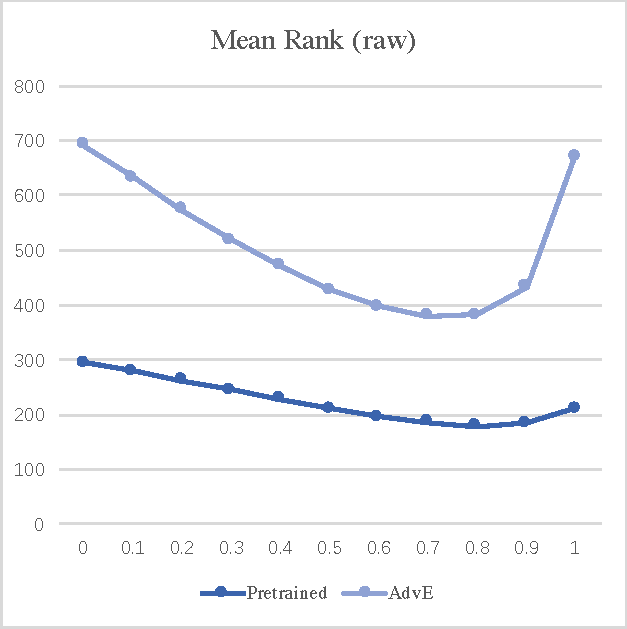
\includegraphics[width=.3\textwidth]{images/ensemble-mean-rank.pdf}
        \subcaption{}        
    }
    \parbox[b]{\columnwidth}{
        \centering
        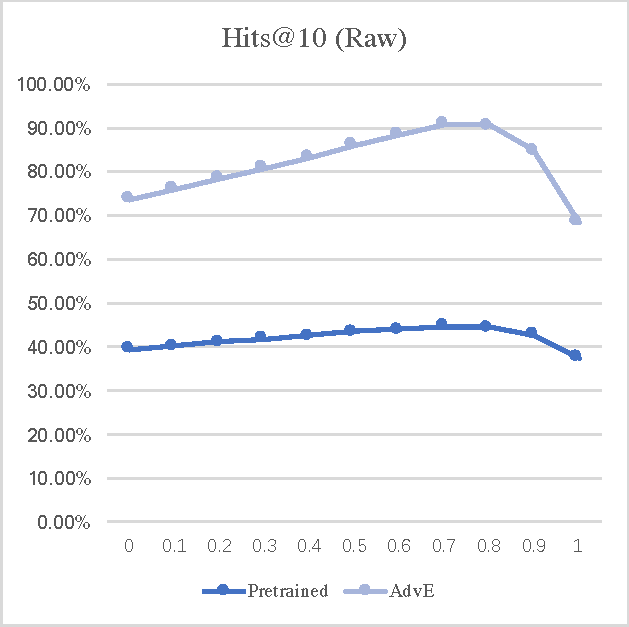
\includegraphics[width=.3\textwidth]{images/ensemble-hit10.pdf}
        \subcaption{}
    }
    \caption{Ensemble parameter selection on validation set. The best alpha value is 0.7 for Hits\@10, and either 0.7 or 0.8 is good for the mean rank metric. Since there isn't much difference on these values, we adopt 0.7 due to the preference for the Hits\@10 metric.}
\label{fig:ensemble}
\end{figure*}

\paragraph{Ensemble Construction} Figure~\ref{fig:ensemble} shows the results of different parameters of ensemble learning on validation set. We conduct ensemble constructions for the pretrained as well as the adversarially trained models. We report the results for both the mean rank and hits@10 metrics under the \emph{raw} criterion. As illustrated in Figure~\ref{fig:ensemble}, a single model, either the generator or the TransE, cannot perform beat the ensemble. According to~(\ref{eq:weighted-ensemble}), $\alpha=0$ shows the performance of the generator only, and $\alpha=1$ the discriminator. The best ensemble $\alpha=0.7$ is in the middle of the two but moderately biased towards TransE.  

\subsection{Triple classification}

blabla

% --------------------------------------
% conclusion

\section{Conclusion}

blabla

% --------------------------------------
\section*{References}


\bibliography{adv-kb2e-bibfile}

\end{document}

% ====================================================
% reference snippets

% \paragraph{Installation} If the document class \emph{elsarticle} is not available on your computer, you can download and install the system package \emph{texlive-publishers} (Linux) or install the \LaTeX\ package \emph{elsarticle} using the package manager of your \TeX\ installation, which is typically \TeX\ Live or Mik\TeX.

% \paragraph{Usage} Once the package is properly installed, you can use the document class \emph{elsarticle} to create a manuscript. Please make sure that your manuscript follows the guidelines in the Guide for Authors of the relevant journal. It is not necessary to typeset your manuscript in exactly the same way as an article, unless you are submitting to a camera-ready copy (CRC) journal.

% \paragraph{Functionality} The Elsevier article class is based on the standard article class and supports almost all of the functionality of that class. In addition, it features commands and options to format the
% \begin{itemize}
% \item document style
% \item baselineskip
% \item front matter
% \item keywords and MSC codes
% \item theorems, definitions and proofs
% \item lables of enumerations
% \item citation style and labeling.
% \end{itemize}

% The author names and affiliations could be formatted in two ways:
% \begin{enumerate}[(1)]
% \item Group the authors per affiliation.
% \item Use footnotes to indicate the affiliations.
% \end{enumerate}
% See the front matter of this document for examples. You are recommended to conform your choice to the journal you are submitting to.